\section{Experiment Design}
In this section we focus on how we design our experiment, implement it with our code, along with our code structure and some fixed bugs.

We fucus on the optimization and simulation of QAOA algorithm and its implementation on the Max-Cut problem in Python. First we implement the QAOA utilizing unitary matrix operator in numpy form. Then we use grid search, Bayesian Optimization and L-BFGS-B to find the best $\beta,\gamma$. With the best  $\beta,\gamma$,we construct its quantum circuits and simulate them both with and without noise using IBM qiskit SDK\cite{Qiskit}. 

\subsection{Data Preparation}
\begin{itemize}
    \item \textbf{graphic\_in.py}: To prepare a random graph with n nodes and get the Max-Cut classic result of it, where \textbf{generateGraph()}  could new a graph and \textbf{graphic(n,edge.ask\_min())} provides its Max-Cut answer as well as division scheme in hexadecimal. The graph will be save into \textbf{grapy\_in.npy}. 
    \item \textbf{graphic\_print.py}: draw the graph using networkx SDK.
\end{itemize}

\subsection{Unitary Matrix Operator Simulation}
In QAOA algorithm, we have 
\begin{align*}
    |\vec{\gamma}, \vec{\beta}\rangle=U(B,\beta_p)U(C,\gamma_p)...U(B,\beta_1)U(C,\gamma_1)|s\rangle 
\end{align*}
where 
\begin{align*}
    U(C, \gamma)=e^{-i\gamma C},U(B, \beta)=e^{-i\beta B}
\end{align*}
which could be achieved by our python code. There are two methods,eigenvalue decomposition and \textbf{np.linalg.eigh} implemention.Eigenvalue decomposition are faster while \textbf{np.linalg.eigh} implemention get better results.


\subsubsection{Eigenvalue Decomposition}
If $C$ is a Hermitian matrix, then it can be diagonalized as $C = UDU^\dagger$, where $U$ is a unitary matrix and $D$ is a diagonal matrix with diagonal elements being the eigenvalues of $C$. Therefore, we can write $e^{-i\gamma C}$ as:
\begin{align*}
    e^{-i\gamma C} = e^{-i\gamma UDU^\dagger}
\end{align*}
Since $U$ is a unitary matrix, it satisfies $UU^\dagger = U^\dagger U = I$. According to the definition of matrix exponential function, we have:
\begin{align*}
    e^{-i\gamma UDU^\dagger} &= \sum_{n=0}^{\infty} \frac{(-i\gamma UDU^\dagger)^n}{n!}\\
    &= \sum_{n=0}^{\infty} \frac{(-i\gamma)^n (UDU^\dagger)^n}{n!}
\end{align*}
Since $U^\dagger U = I$, $(UDU^\dagger)^n = UD^nU^\dagger$. Therefore, we can write the above formula as:
\begin{align*}
    e^{-i\gamma UDU^\dagger} &= \sum_{n=0}^{\infty} \frac{(-i\gamma)^n UD^nU^\dagger}{n!} \\
    &= U\left(\sum_{n=0}^{\infty} \frac{(-i\gamma)^n D^n}{n!}\right)U^\dagger \\
    &= Ue^{-i\gamma D}U^\dagger
\end{align*}

Therefore, by performing eigenvalue decomposition on $C$, we can transform the calculation of matrix exponential function into direct calculation of diagonal elements. In this way, we can avoid the error of matrix exponential function. However, the precision of eigenvalue decomposition obtained by \textbf{np.linalg.eig} cannot meet the requirements. Its error is so significant that the result of $e^{-i\gamma C}$ is no longer an unitary matrix any more. By multipling these so-called unitary matrix, the magnitude of the final state $|\vec{\gamma}, \vec{\beta}\rangle $ is far away from 1. It's the first \textbf{precision disasters} we have met. When we use tried different $\vec{\gamma}, \vec{\beta} $ in optimization section to get best parameters, sometimes we got dramatical results like $F_p$ larger than 10000.  To solve the problem, we finally discover this precision bug.  So we used \textbf{np.linalg.eigh} for eigenvalue decomposition to achieve the better precision. 




\subsubsection{Expm Direct Calculation}
Since the method of eigenvalue decomposition doesn't work, we are forces to seek other solutions,which leads us to \textbf{scipy.linalg.expm}. We analyse its result, which turn out to be a nice one. We find $e^{-i\gamma C}$ is an unitary matrix and the magnitude of the final state $|\vec{\gamma}, \vec{\beta}\rangle $ is about 0.9999, which is a satisfactory result. So we choose the new method and solve the first \textbf{precision disasters}.

\subsection{Parameter Optimization}

Now, given an array of $|\vec{\gamma}, \vec{\beta}\rangle$, We could simulate the QAOA. So we try to find the best array of $|\vec{\gamma}, \vec{\beta}\rangle$ at fixed $p$. That's exactly what we do in \textbf{optimize.ipynb}, finding best array of $|\vec{\gamma}, \vec{\beta}\rangle$ at fixed $p$ and n with various methods.

We use dfs to achieve the grid search, hyperopt package\cite{bergstra2013making} to finish Bayesian Optimization and scipy. optimize to implement basinhopping algorithm in L-BFGS-B method. We compare these three algorithm using its $F_p$. 
\begin{align*}
    F_p(\vec{\gamma}, \vec{\beta}) = \langle\vec{\gamma},\vec{\beta}| C |\vec{\gamma},\vec{\beta}\rangle
\end{align*}

According to our test result shown as TABLE.\ref{tab:Opt}, it turns out that basinhopping and L-BFGS-B have done a faster and better job. 

We want to find out how $F_p$ changes as $p$ increases in two fixed graphs shown as FIG.\ref{fig:n=7} and FIG.\ref{fig:n=8}. So we iterate $p$ in $range(1,11)$  and utilize basinhopping algorithm in L-BFGS-B method to optimize the $F_p$  for each $p$. Then we get the result of each $p$ and save the $\vec{\gamma},\vec{\beta}$. And the formulation of accuracy we use here is 
\begin{align*}
    \text{Accuracy}=\frac{F_p(\vec{\gamma}, \vec{\beta})}{\text{Answer of classical Algorithm}}
\end{align*}


We tried to run as large n as possible. However, as n increase 1,the unitary matrix times 4 and it will take more attempts in parameter fine-tuning process.At last we chose n=8 and generate a graph as shown in FIG.\ref{fig:n=8}. We run on Lab's \textit{Intel(R) Xeon(R) Gold 6226R CPU @ 2.90GHz} and it takes us several days to get the final result.

\begin{figure}[!htb]
    \centering
    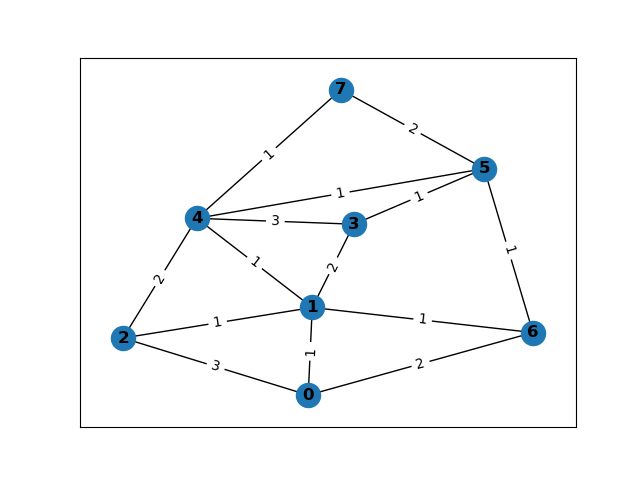
\includegraphics[width=0.309\textwidth]{graphic_n=8.png}
    \caption{An Graphic Example of n=8,whose Max Cut = 19}
    \label{fig:n=8}
\end{figure}

However,when we attempt simulate the quantum circuit, we find out that we could only simulate quantum circuit with noise in n=7 utlizing qiskit, since the free IBM quantum machine has a maxium qubit of 7 and we use its noise data.Since quantum circuit simulation needs the optimized $\vec{\gamma},\vec{\beta}$,we generate a new graph, shown as FIG.\ref{fig:n=7}, and repeat the above process.

\begin{figure}[!htb]
    \centering
    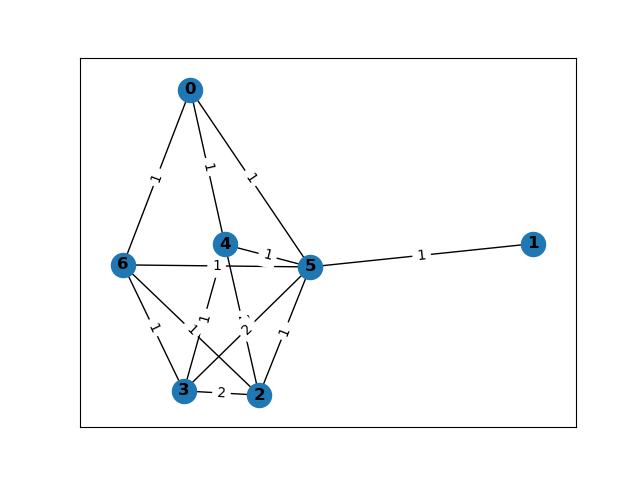
\includegraphics[width=0.309\textwidth]{graphic_n=7.png}
    \caption{An Graphic Example of n=7,whose Max Cut = 11}
    \label{fig:n=7}
\end{figure}

\clearpage

\subsection{Quantum Circuits Simulation}

We prepare our qubits with an Hadamard Gate to obtain the mixed state. $U(C, \gamma)=e^{-i\gamma C}$ could be achieved by applying a $Rz(-\gamma)$ and two $C_x$ gate at  both ends of it.  $U(B, \beta)=e^{-i\beta B}$ could be simply implemented deploying $R_x(2\beta)$ gate. In this way, we succeed in constructing the quantum circuit. Our code could be run on quantum machines,but the long waiting list prevent us. The typical quantum circuit our code generated is shown as FIG.\ref{fig:expamle circuit}. The datasheet of ibm nairobi,the real quantum machine we simulate, is shown in FIG.\ref{fig:overview of ibm_nairobi}.

\begin{figure}[!htb]
    \centering
    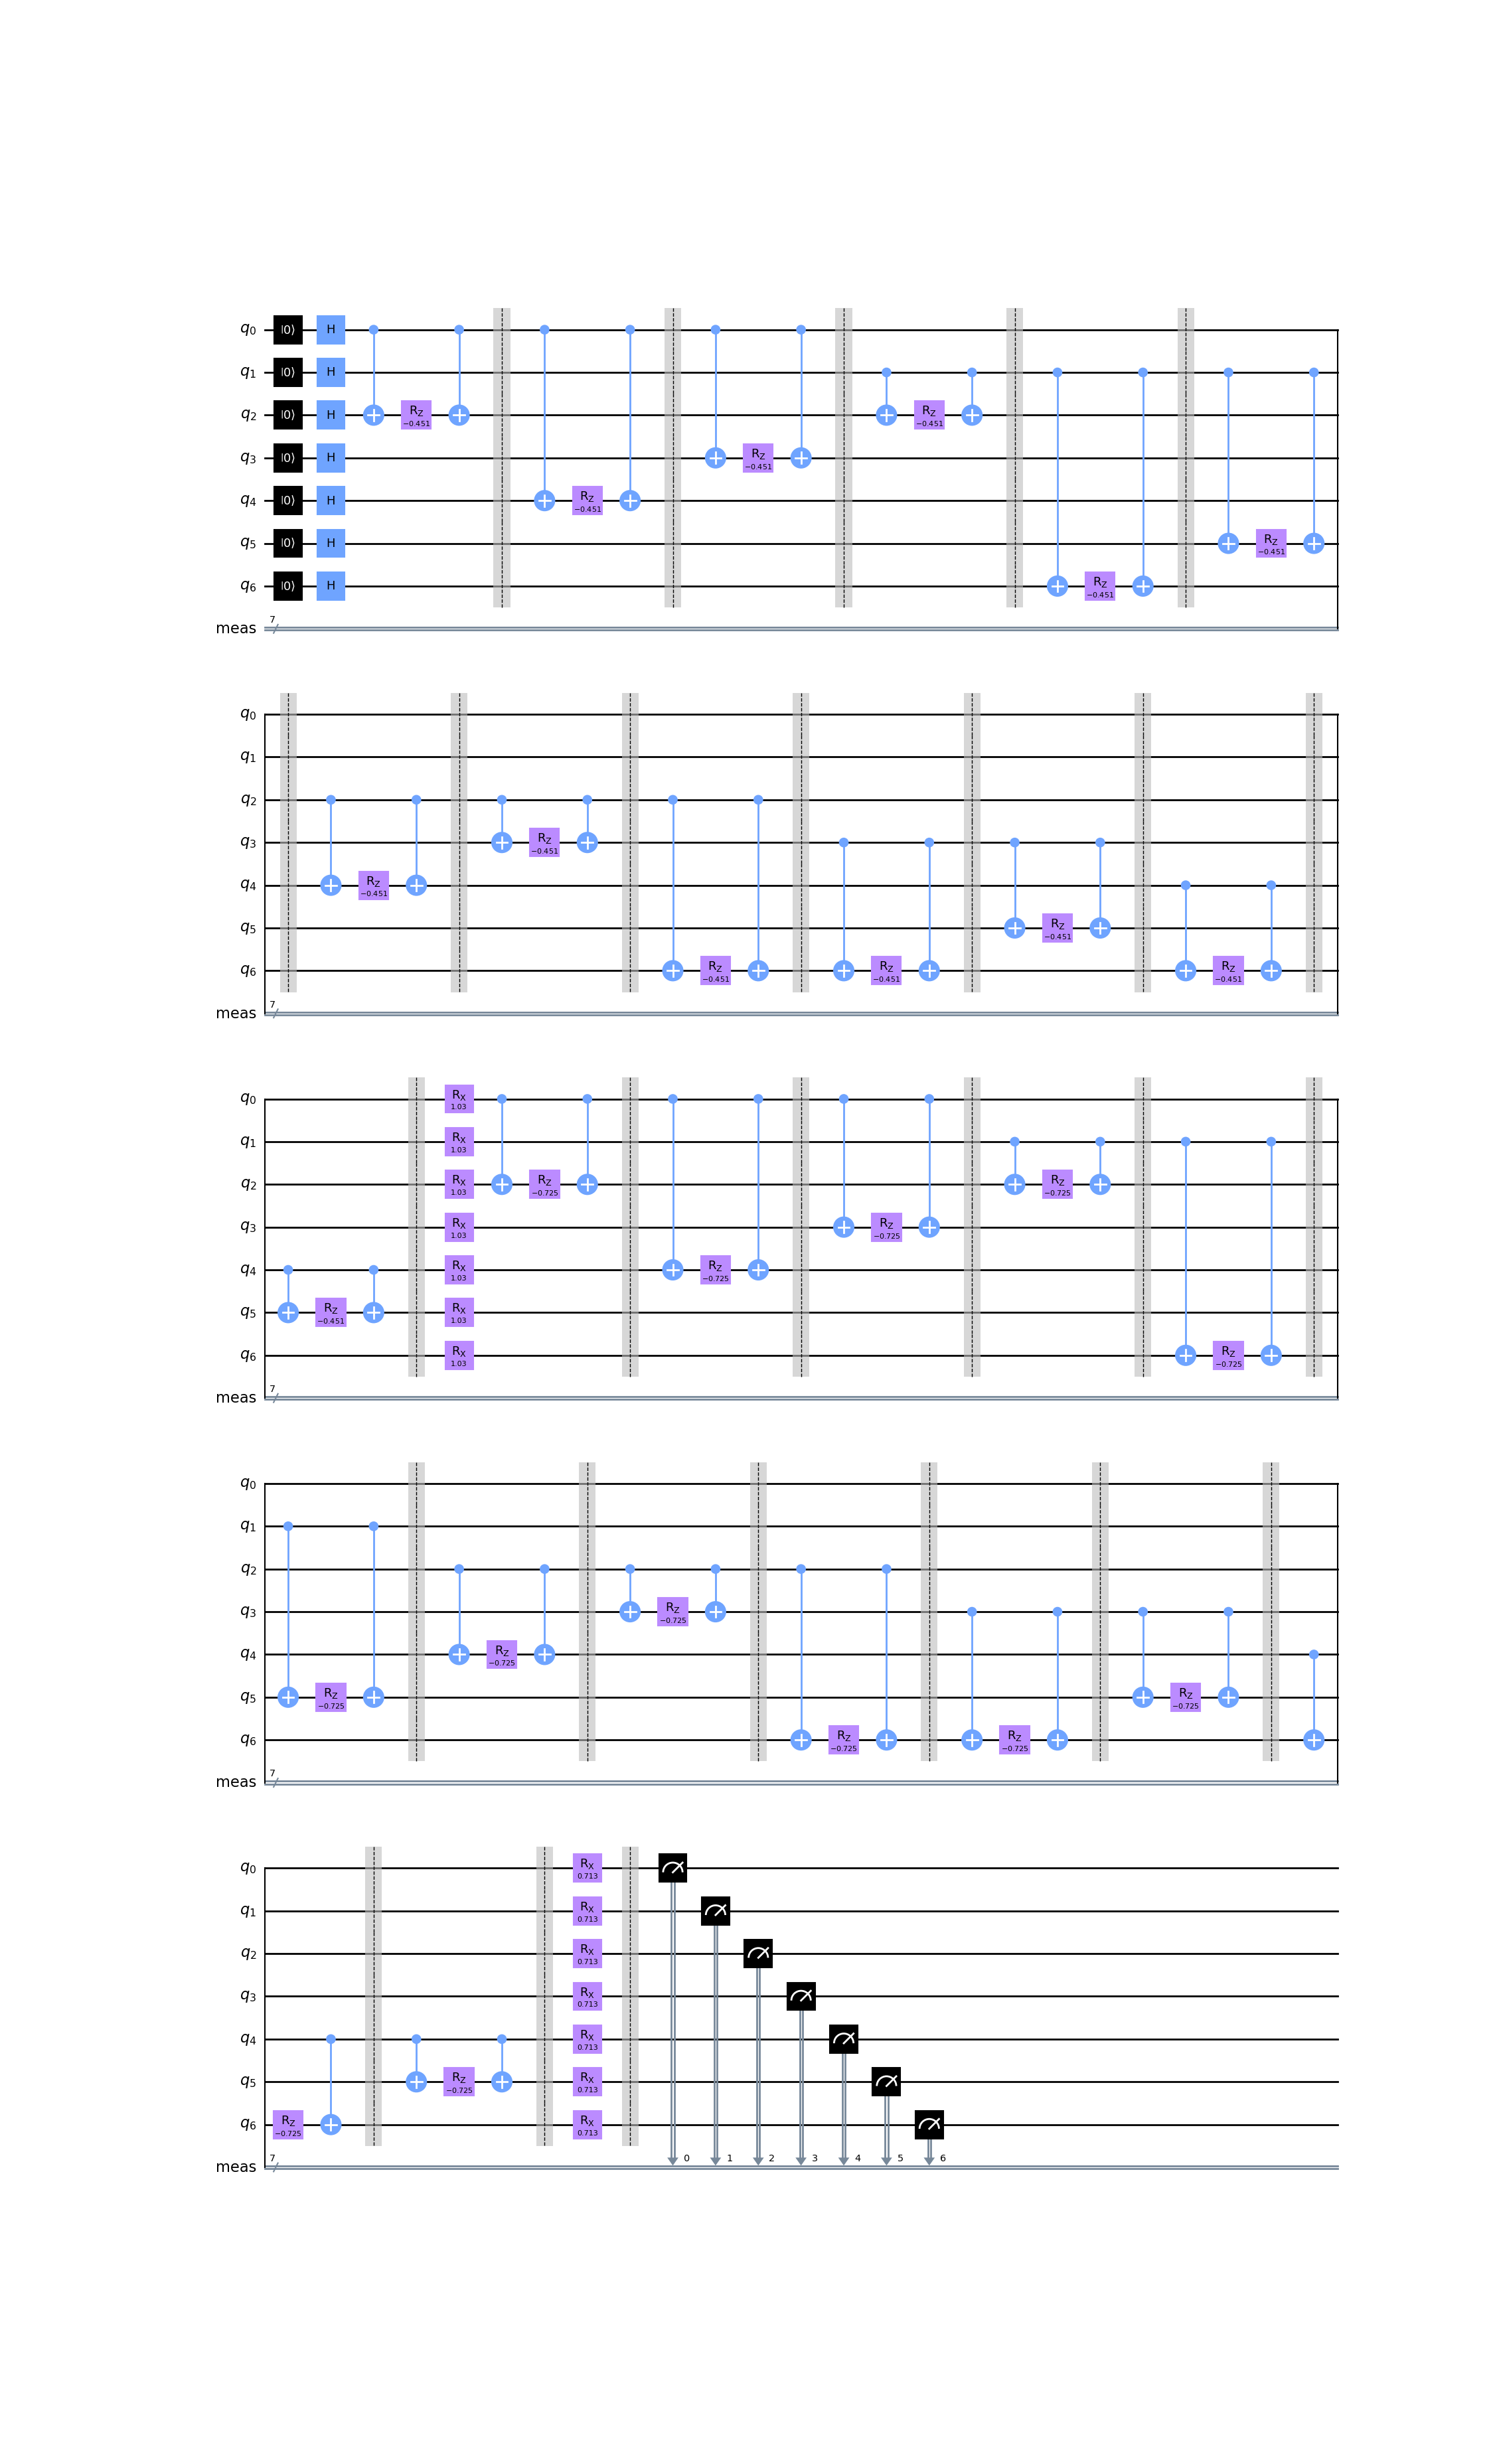
\includegraphics[width=0.3\textwidth]{circuit.png}
    \caption{A quantum circuit example at n=7,p=2.}
    \label{fig:expamle circuit}
\end{figure}

\begin{figure}[!htb]
    \centering
    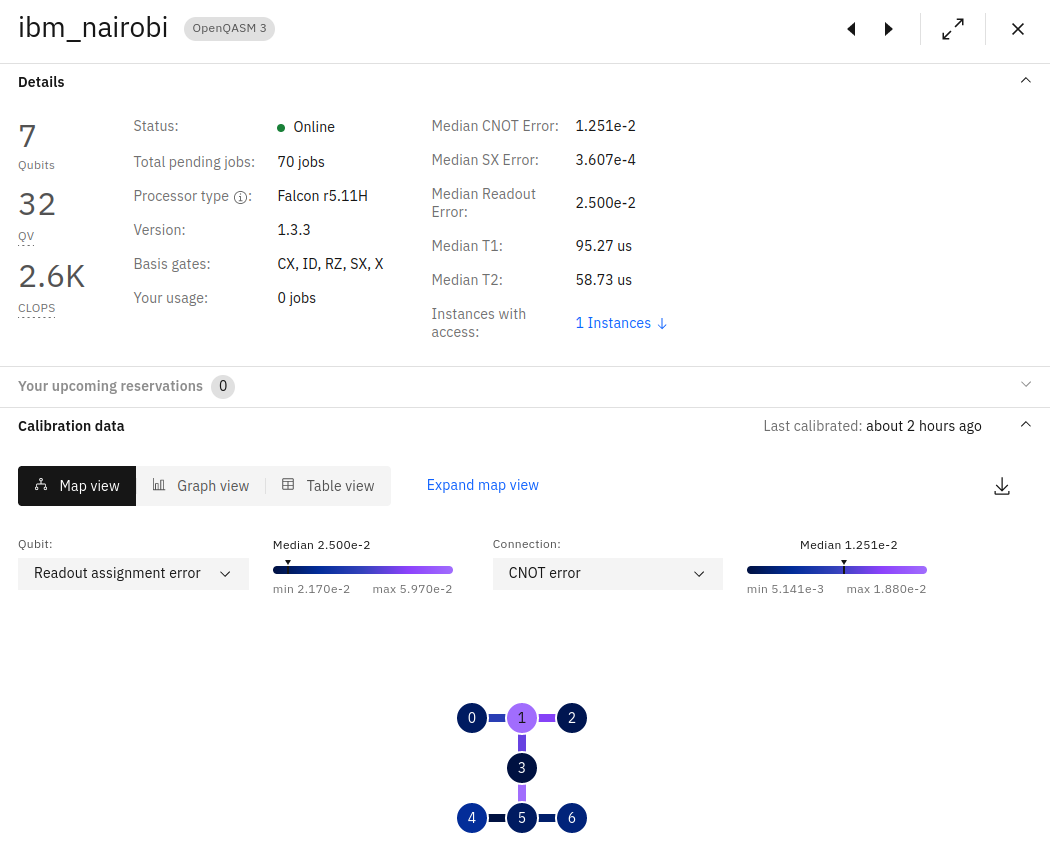
\includegraphics[width=0.42\textwidth]{overview of ibm_nairobi.png}
    \caption{Overview of ibm nairobi}
    \label{fig:overview of ibm_nairobi}
\end{figure}

\begin{figure}[!htb]
    \centering
    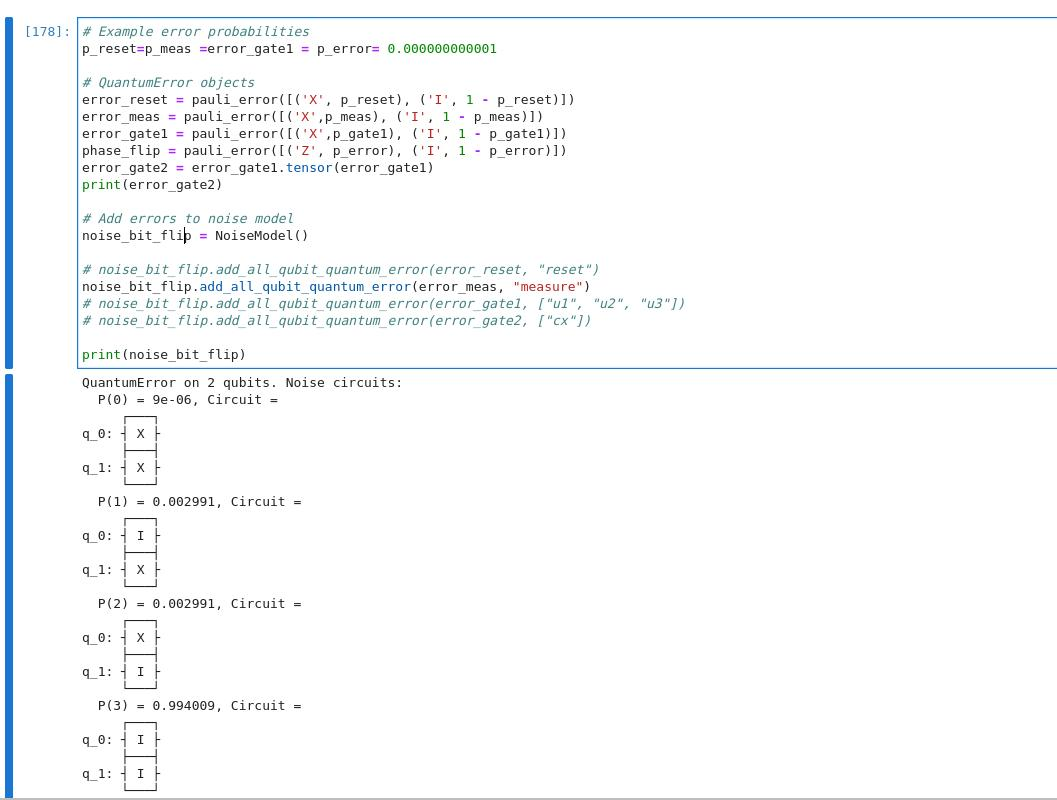
\includegraphics[width=0.3\textwidth]{failure.jpg}
    \caption{A Failed Attempt to Construct the $R_z$ Error}
    \label{fig:failure}
\end{figure}

We obtain our result both with and without noise with the help of \textbf{qasm\_simulator}. We draw the top 5 states of each situation in the same histogram for $p$ in $range(1,7)$. We try the original 1024 shots shown results in FIG.\ref{fig:1024-shots} and the large enough 100000 shots  shown results in FIG.\ref{fig:100000-shots}, which we aim to observe the real quantum computation result and the expectation of the final states individually. At the same time, we plot the Accuracy-p figure with and without noise, to help us better understand the influence of noise. 
\begin{align*}
    \text{Accuracy}=\frac{\text{number of desired states}}{\text{total shot number}}
\end{align*}

Besides, in the experiment we attempt to construct the $R_z$ error ourself, which turn out to be another precision disasters. As show in the FIG.\ref{fig:failure}, we set the possibility of error to zero, but we still obtain an undesired gate result.(It's $P(1)$ is obviously not zero and its $P(3)$ is not 1.) We failed to fix this precision bug. That's why we turn to actual quantum machine noise data.




\subsection{Experiment Design summary}
\begin{enumerate}
    \item We implement QAOA on Max-Cut using  unitary matrix operator.
    \item We tried three different ways of parameters optimization and test them with various n and p to find out the pros and cons.
    \item We construct the quantum circuit of QAOA.
    \item We simulate the quantum circuit using qiskit and use real quantum machine's error data to simulate the noise.
    \item We plot our experiment result and discuss the reason behind it.
\end{enumerate}
\clearpage
\section{Experiment Result and Analyse}

\subsection{Comparison of different optimizor}

TABLE.\ref{tab:Opt} compares the performances of different optimizer on data with different attributes. It is shown that when $p=1, 2$, the result of brute force is relatively not bad. However, as $p$ increases, the brute force algorithm takes too long to execute and the Bayes algorithm meets difficulty in accuracy. BFGS algoririthm remains the most stable one.

The result also shows that the accuracy grow significantly with $p$ when $p$ is not so large.

\begin{table}[htbp]
  \centering
  \caption{Optimizor}
    \begin{tabular}{lrrrrrr}
\toprule
          & \multicolumn{3}{c}{n=7, p=1, k=20} & \multicolumn{3}{c}{n=7, p=2, k=10} \\
\midrule
    real answer & 8     & 3     & 9     & 4     & 15    & 8 \\
    Bayes  & 6.299  & 2.357  & 7.271  & 3.384  & 13.209  & 6.274  \\
    BFGS  & 6.307  & 2.380  & 7.336  & 3.122  & 13.601  & 6.696  \\
    brute force & 6.140  & 2.337  & 7.213  & 3.343  & 11.860  & 6.043  \\
    BFGS ratio & 0.788  & 0.793  & 0.815  & 0.781  & 0.907  & 0.837  \\
\midrule
          & \multicolumn{3}{c}{n=7, p=3} & \multicolumn{3}{c}{n=7, p=4} \\
\midrule
    real answer & 12.000  & 8.000  & 11.000  & 15.000  & 14.000  & 13.000  \\
    Bayes  & 9.933  & 5.693  & 8.154  &       &       &  \\
    BFGS  & 11.100  & 6.698  & 9.218  & 14.041  & 12.726  & 11.817  \\
    BFGS ratio & 0.925  & 0.837  & 0.838  & 0.936  & 0.909  & 0.909  \\
\bottomrule
    \end{tabular}%
   \label{tab:Opt}%
\end{table}%

\subsection{Parameter Optimization}
We are interested in how the $F_p$ of a certain graph develops as p grows.

\begin{figure}[!htb]
    \centering
        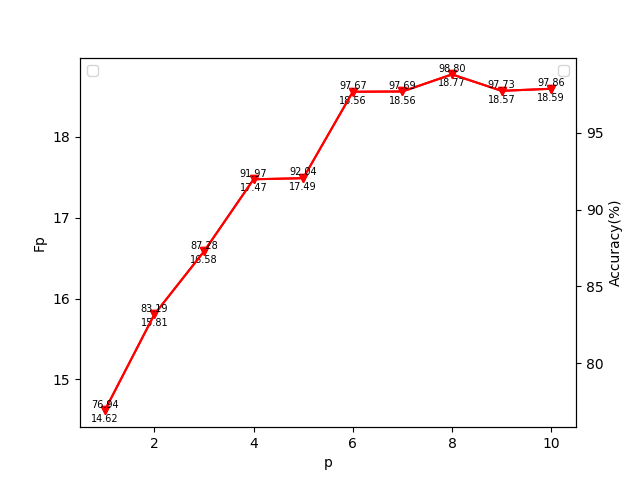
\includegraphics[width=0.4\textwidth]{pic/result_8.png}
        \caption{The relationship between $F_p$ and $p$ , $n=8$}
    \label{fig:result_8}
\end{figure}

First,we run our algorithm at n=8,shown as FIG.\ref{fig:n=8} and we got the result as FIG.\ref{fig:n=8}. For p larger than 6,we achieve an accuracy of 97\%,which is really impressive. Some fluctuation occurs when p is large. It's because our optimization algorithm may have stuck in the local minima sometimes. 

Then,we run our algorithm at n=7,shown as FIG.\ref{fig:n=7} and we got the result as FIG.\ref{fig:n=7}. We even achieve an accuracy of 99.86\%! Since n is smaller, we got a smooth monotonically increasing curve this time.
\begin{figure}[!htb]
    \centering
        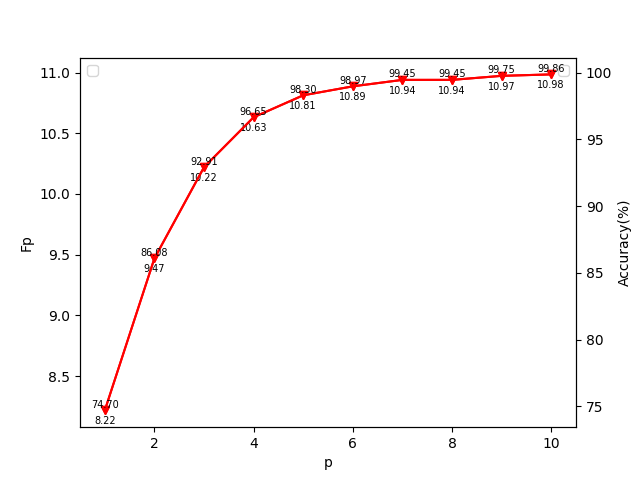
\includegraphics[width=0.4\textwidth]{pic/result_7.png}
        \caption{The relationship between $F_p$ and $p$ on the fixed graph with $n=7$ vertices}
    \label{fig:result_7}
\end{figure}


Besides, it's worth mention that since p refer to the time our edges could expand to its neighbors, the longest path in the solution graph at $p$ is $2p+1$\cite{farhi2014quantum}, which means final solution may be unachievable for small p in theroy. 

In conclusion, the experiment result shows that $F_p$ increases as $p$ increases and 
\begin{align*}
    \lim_{p\rightarrow \infty}\max_{\vec{\gamma}, \vec{\beta}}{F_p(\vec{\gamma}, \vec{\beta})}=C_{max}(z)
\end{align*}







\subsection{Quantum Circuits Simulation}


The top-5 quantum circuit's result states histogram pictures are shown in FIG.\ref{fig:1024-shots} and FIG.\ref{fig:100000-shots}, 1024 shots situation and 100000 shots situation correspondingly.
%\clearpage
\begin{figure*}[!htb]
    \centering
    \subfloat[1024 shots]{
        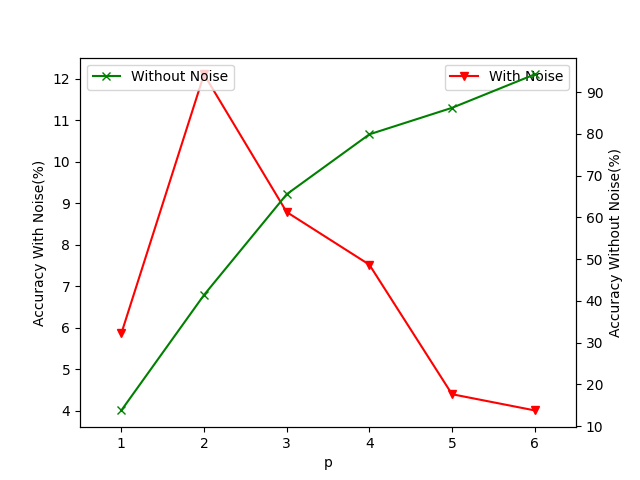
\includegraphics[width=0.42\textwidth]{result/[shots=1024]Accuracy-P}
    }
    \subfloat[100000 shots]{
        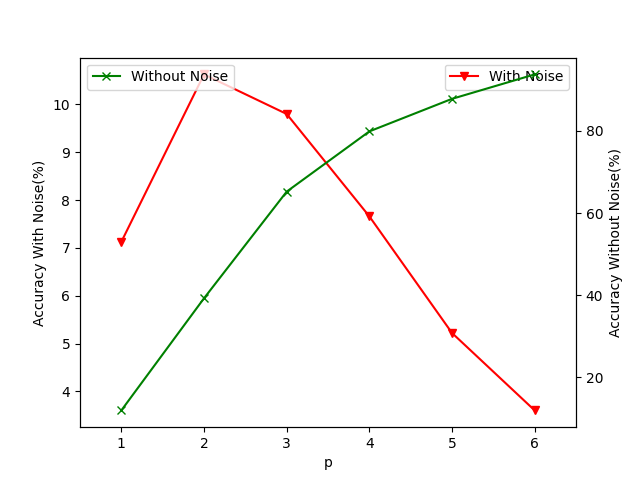
\includegraphics[width=0.42\textwidth]{result/Accuracy-P}
    }
    \caption{Accuracy-P digram}
    \label{fig:Accuracy-P}
\end{figure*}

\begin{figure*}[!htb]
    \centering
    \begin{minipage}{\textwidth}
        \centering
        \subfloat[$P=1$]{
            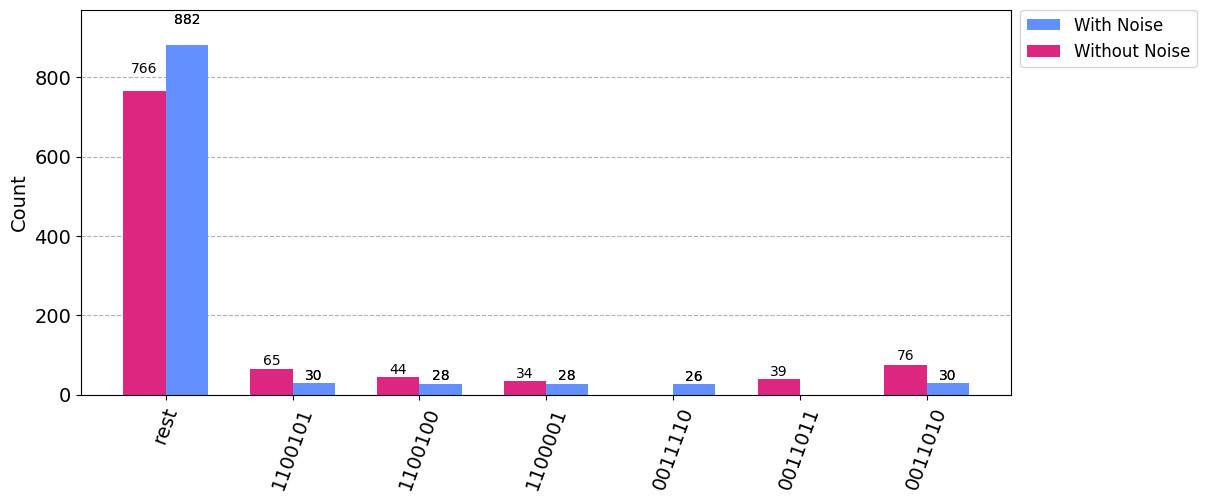
\includegraphics[width=0.3\textwidth]{result/[shots=1024]P=1}
        }
        \subfloat[$P=2$]{
            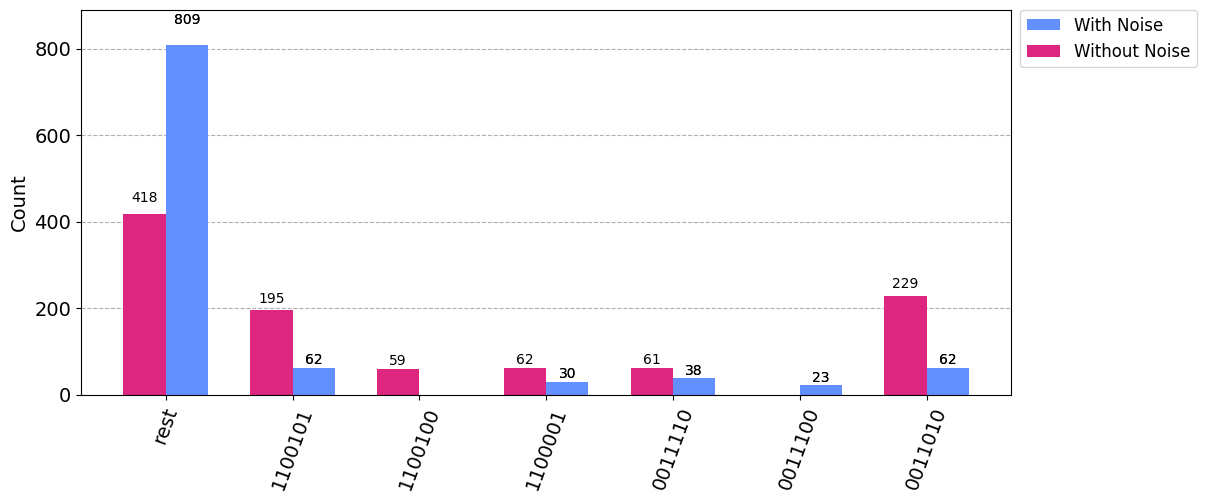
\includegraphics[width=0.3\textwidth]{result/[shots=1024]P=2}
        }
        \subfloat[$P=3$]{
            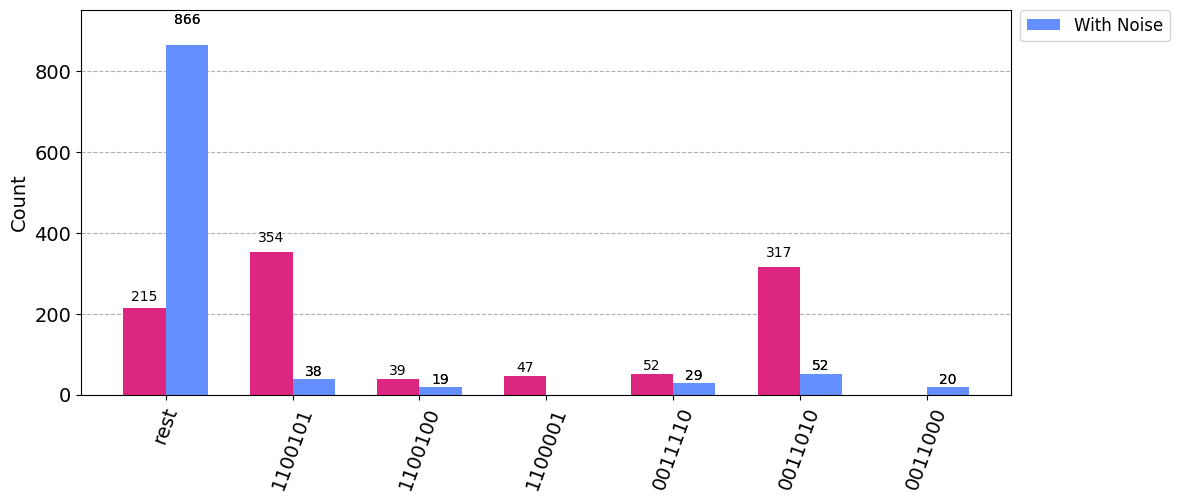
\includegraphics[width=0.3\textwidth]{result/[shots=1024]P=3}
        }
    
        \subfloat[$P=4$]{
            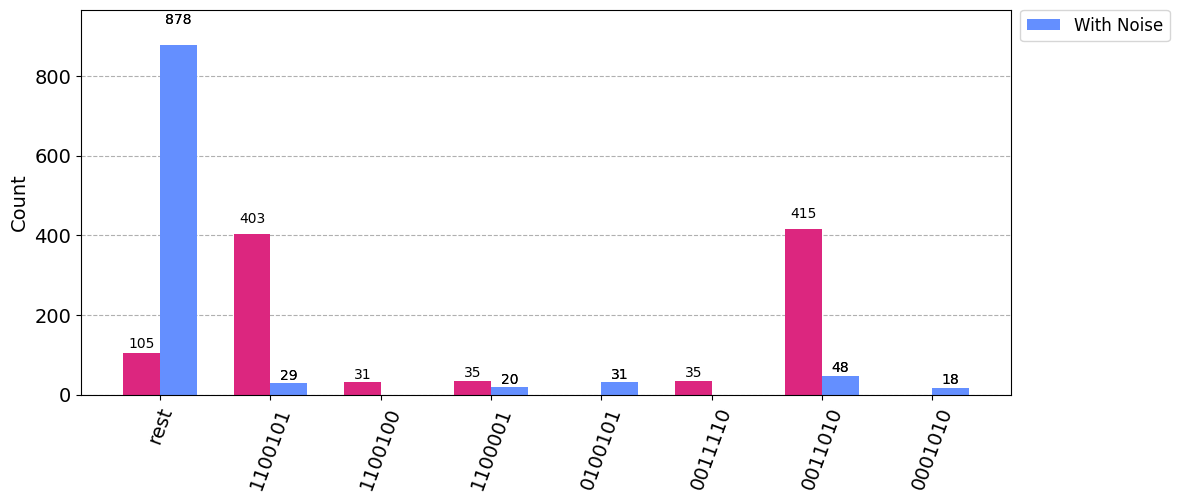
\includegraphics[width=0.3\textwidth]{result/[shots=1024]P=4}
        }
        \subfloat[$P=5$]{
            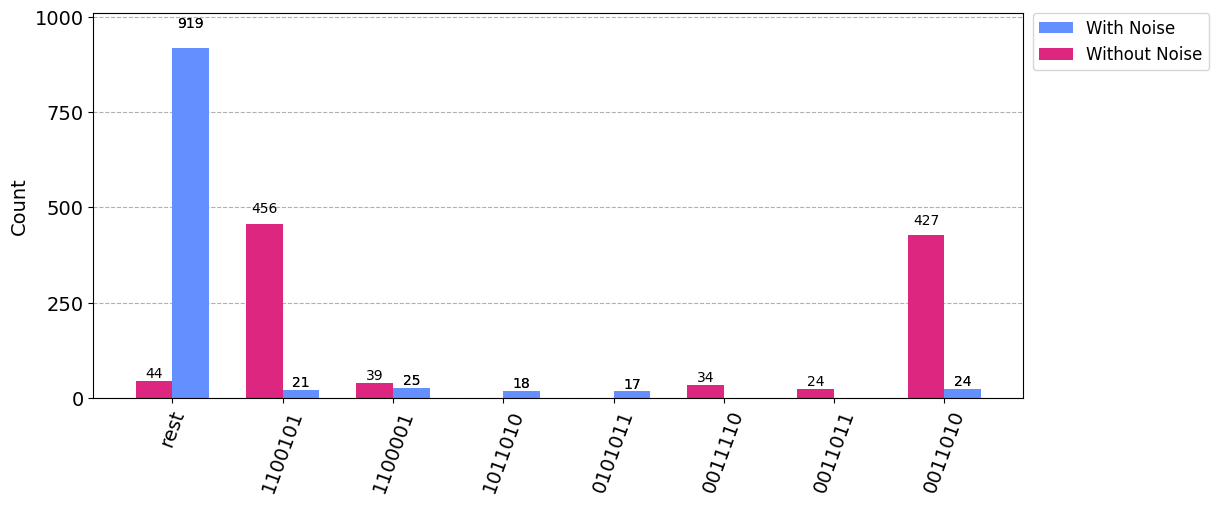
\includegraphics[width=0.3\textwidth]{result/[shots=1024]P=5}
        }
        \subfloat[$P=6$]{
            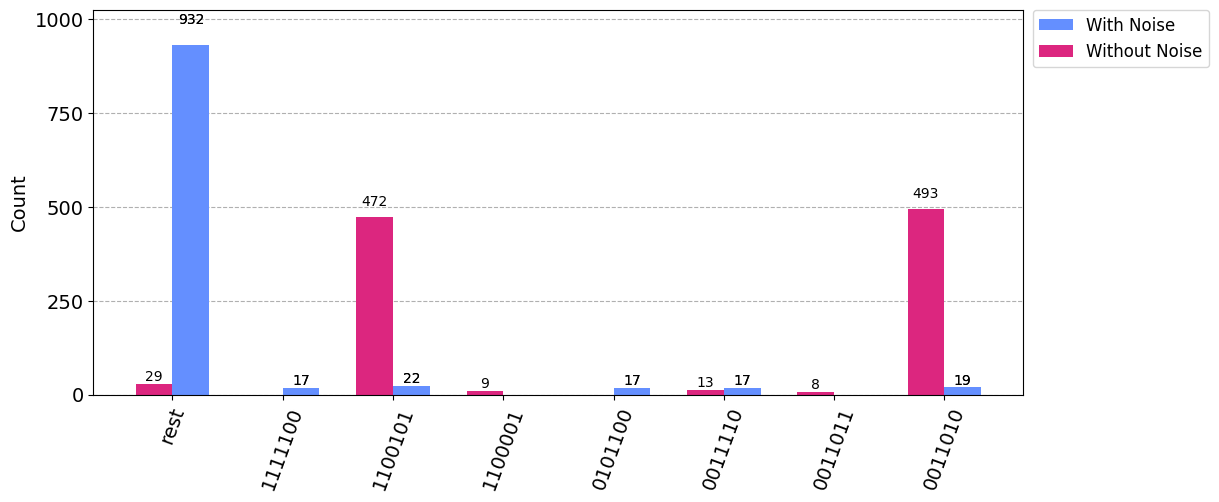
\includegraphics[width=0.3\textwidth]{result/[shots=1024]P=6}
        }
        \caption{Output tates statistics for different p at 1024 shots}
        \label{fig:1024-shots}
    \end{minipage}

    \begin{minipage}{\textwidth}
        \centering
        \subfloat[$P=1$]{
            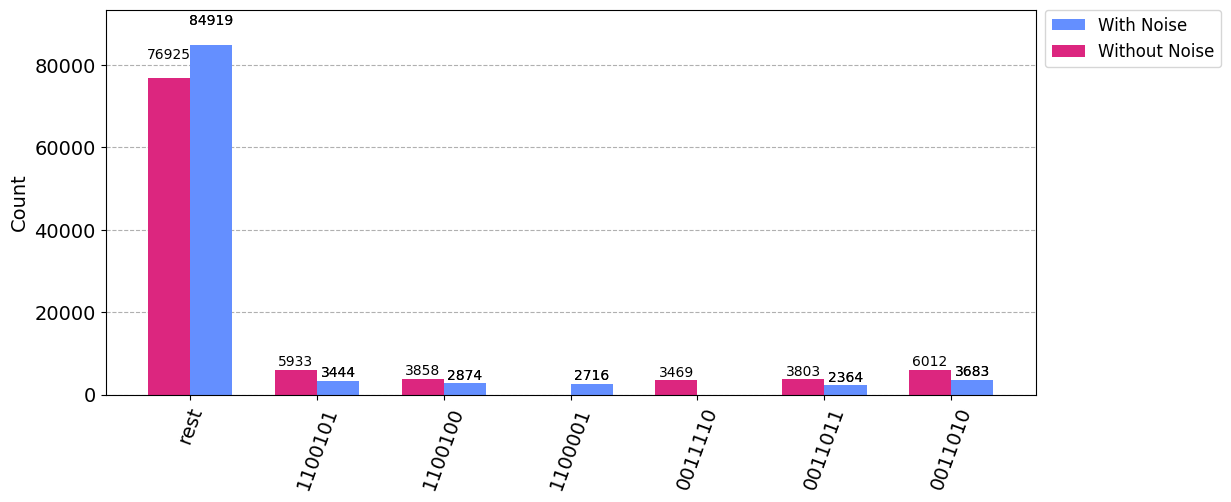
\includegraphics[width=0.3\textwidth]{result/P=1}
        }
        \subfloat[$P=2$]{
            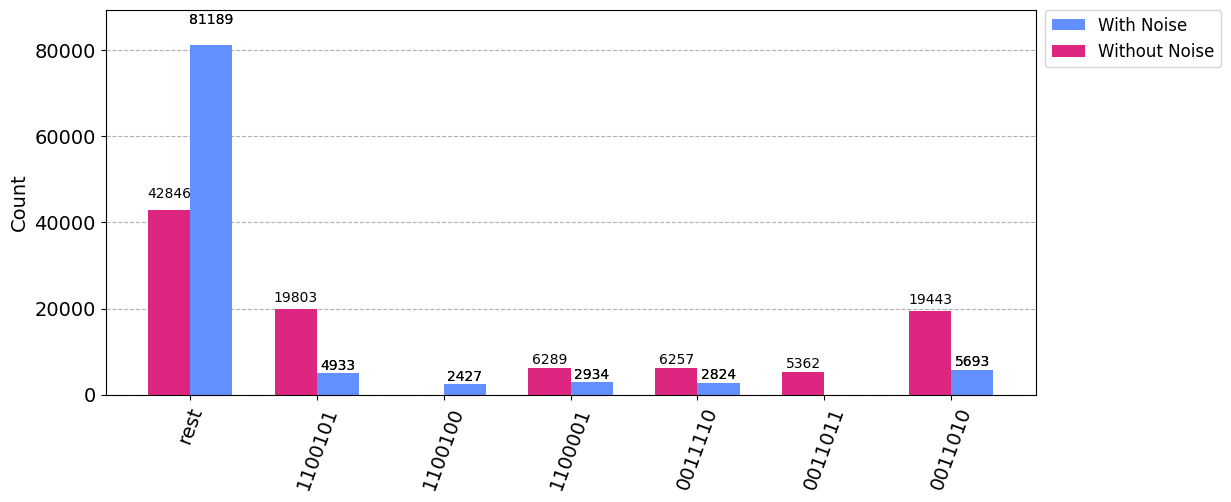
\includegraphics[width=0.3\textwidth]{result/P=2}
        }
        \subfloat[$P=3$]{
            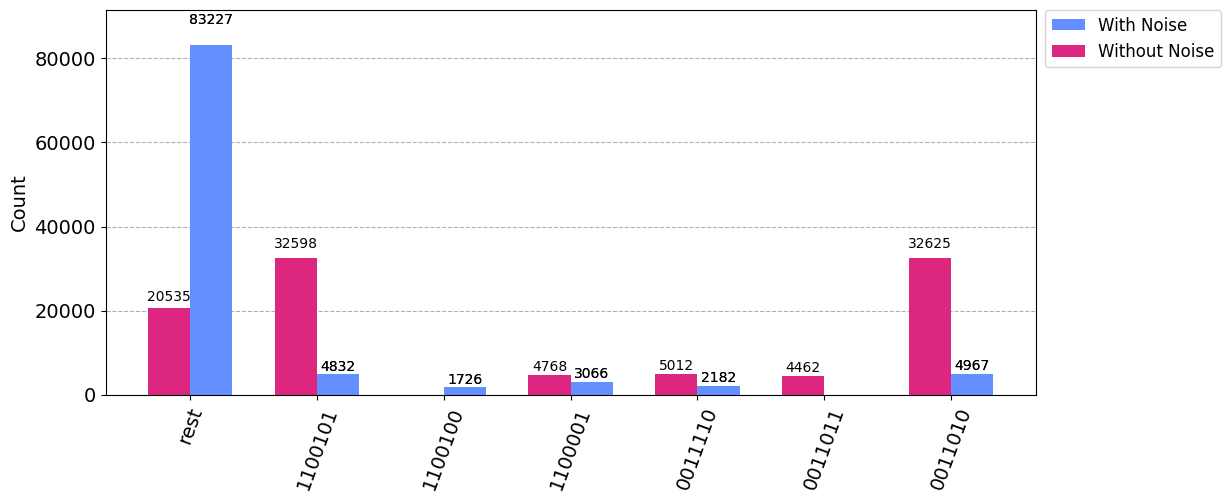
\includegraphics[width=0.3\textwidth]{result/P=3}
        }
    
        \subfloat[$P=4$]{
            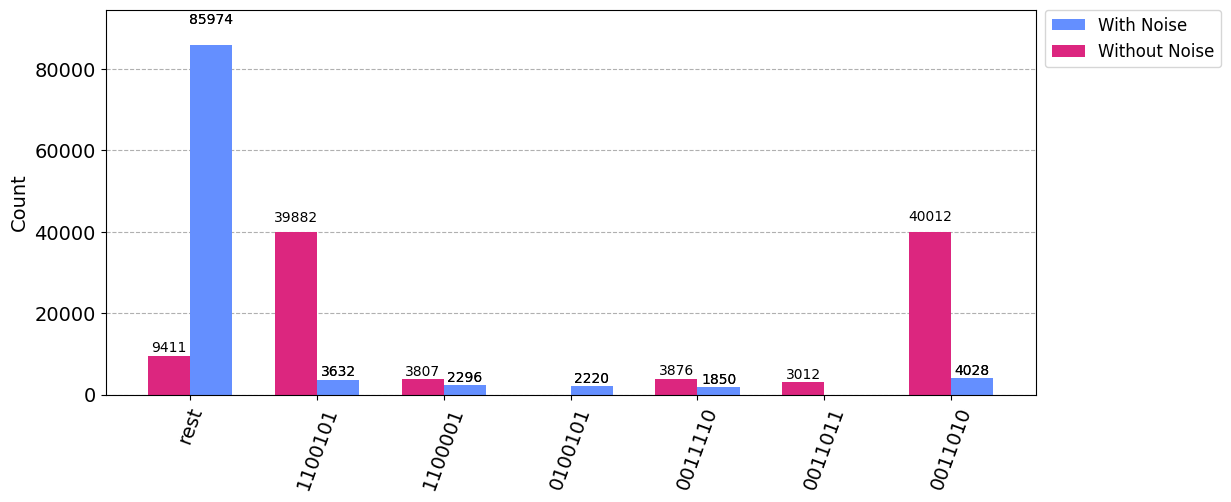
\includegraphics[width=0.3\textwidth]{result/P=4}
        }
        \subfloat[$P=5$]{
            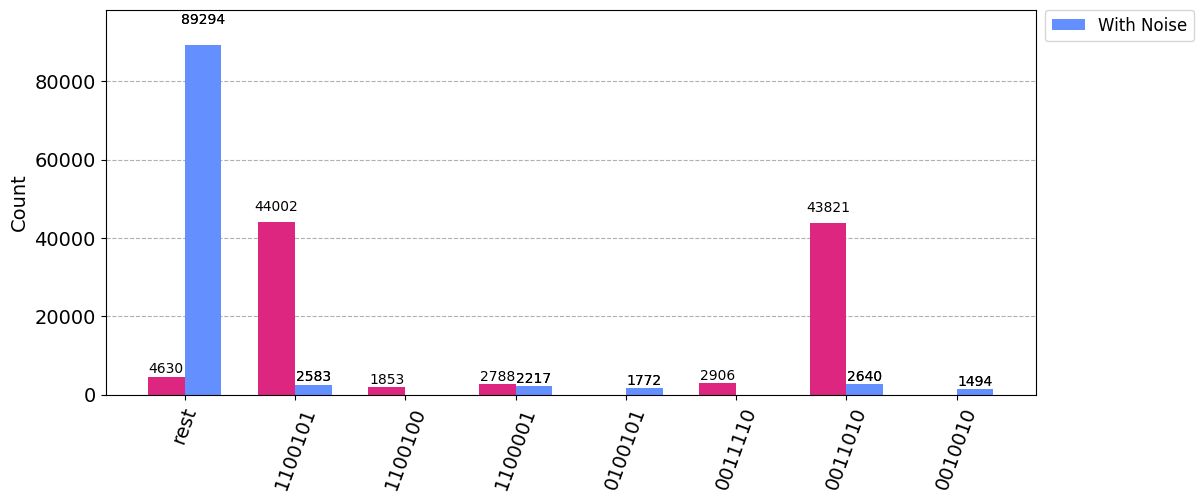
\includegraphics[width=0.3\textwidth]{result/P=5}
        }
        \subfloat[$P=6$]{
            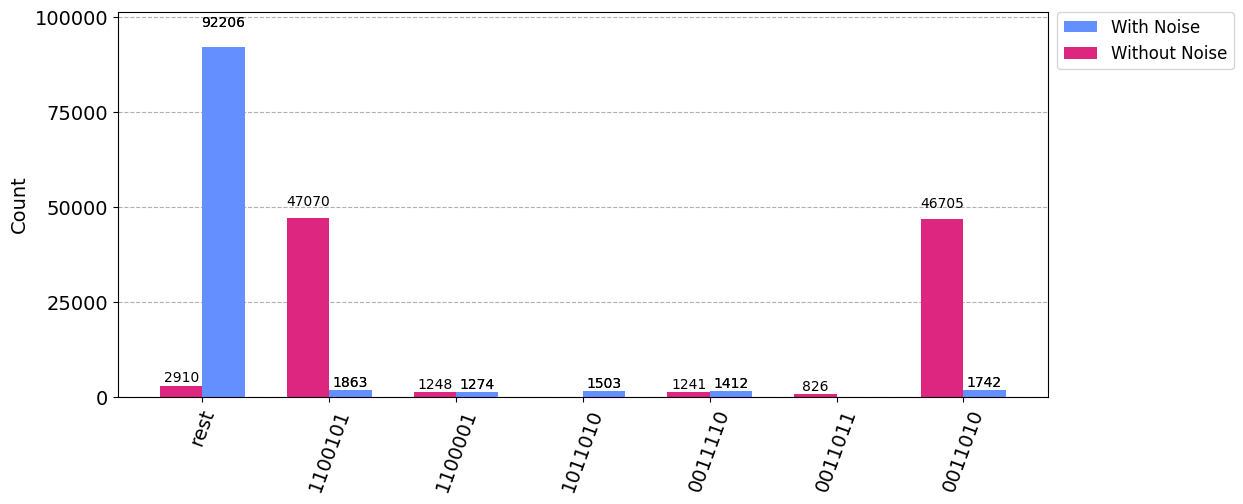
\includegraphics[width=0.3\textwidth]{result/P=6}
        }
        \caption{Output tates statistics for different p at 100000 shots}
        \label{fig:100000-shots}
    \end{minipage}
\end{figure*}
\clearpage
We will find that for shots=100000 in FIG.\ref{fig:Accuracy-P}, the accuracy states could always be distinguished,though hard. So the noise only decrease the possibility of our desired states  and randomly attribute them with others states. Since the same process act on every states, the possibility of our desired states are still ahead of others,though the gap is getting smaller as the depth of the quantum circuit increase.

However,for shots=1024,they could only be figured out at $p=2$ and 3. It's due to the random nature of quantum measurement. As long as the expectation two states are close, they will mix up easily. So in practical, we must control the depth of the quantum circuit since the random nature of quantum measurement may bridge the gap between our desired states and others.

As we analyze Accuracy-p figure in FIG.\ref{fig:1024-shots} and  FIG.\ref{fig:100000-shots}, it's easy to obtain that noise dramatically decrease the accuracy. As $p$ increases, the depth of quantum circuit increases,leading to more noise and less accuracy. 

Besides, although  accuracy increase with $p$ for noiseless situation just as it's theoretically proved , the noise effect will over weigh the accuracy improvement of $p$ and become dominate for sufficient large $p$ (in this case $p=2$). That's why accuracy first increase then decrease as $p$ increases.

So we should carefully choose our p when we deploy QAOA in real quantum machine.




% \begin{figure*}[!htbp]
%     \centering
%     \subfloat[$P=1$]{
%         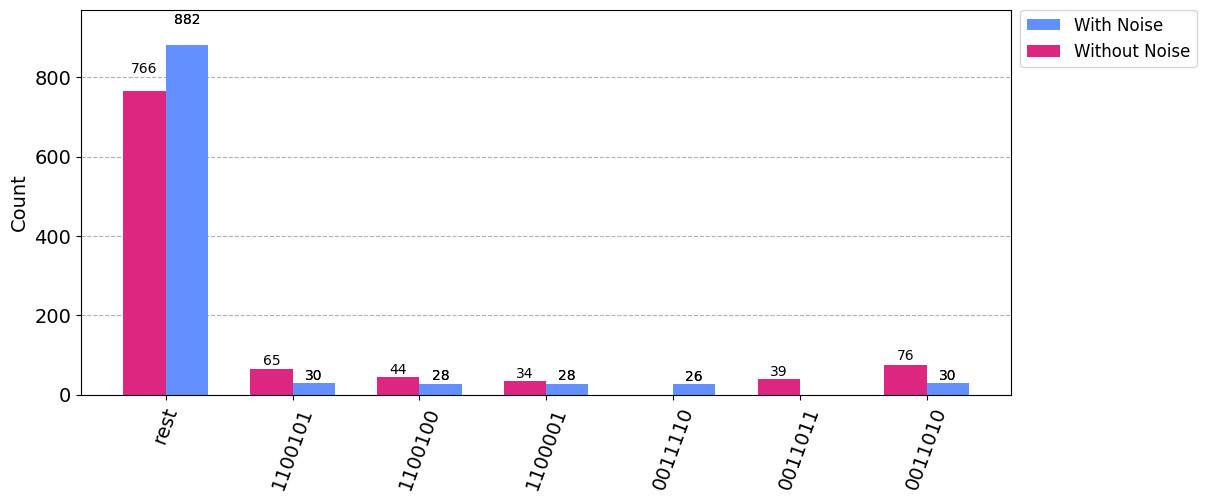
\includegraphics[width=0.5\textwidth]{result/[shots=1024]P=1}
%     }
%     \subfloat[$P=2$]{
%         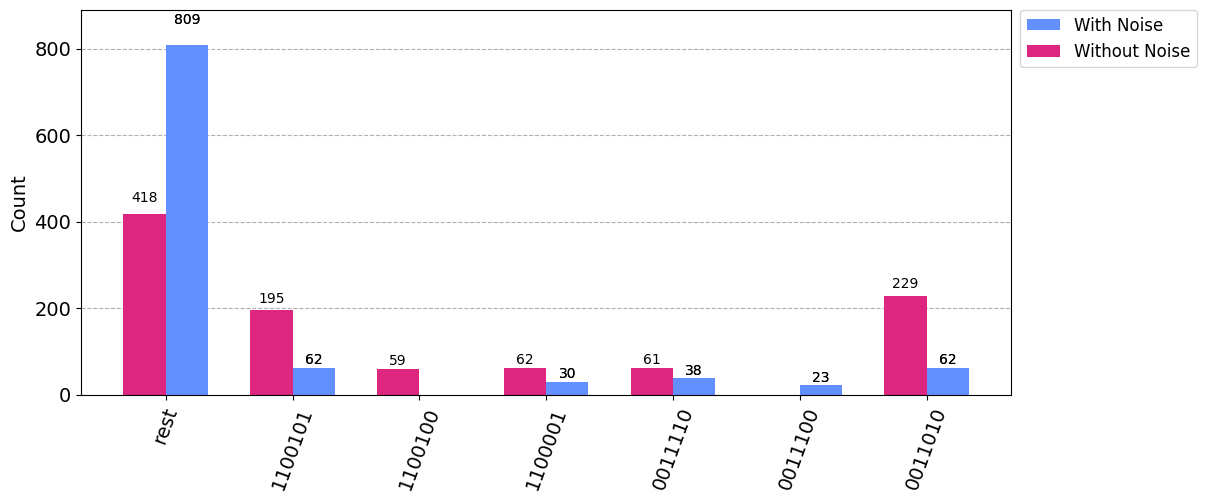
\includegraphics[width=0.5\textwidth]{result/[shots=1024]P=2}
%     }
    
%     \subfloat[$P=3$]{
%         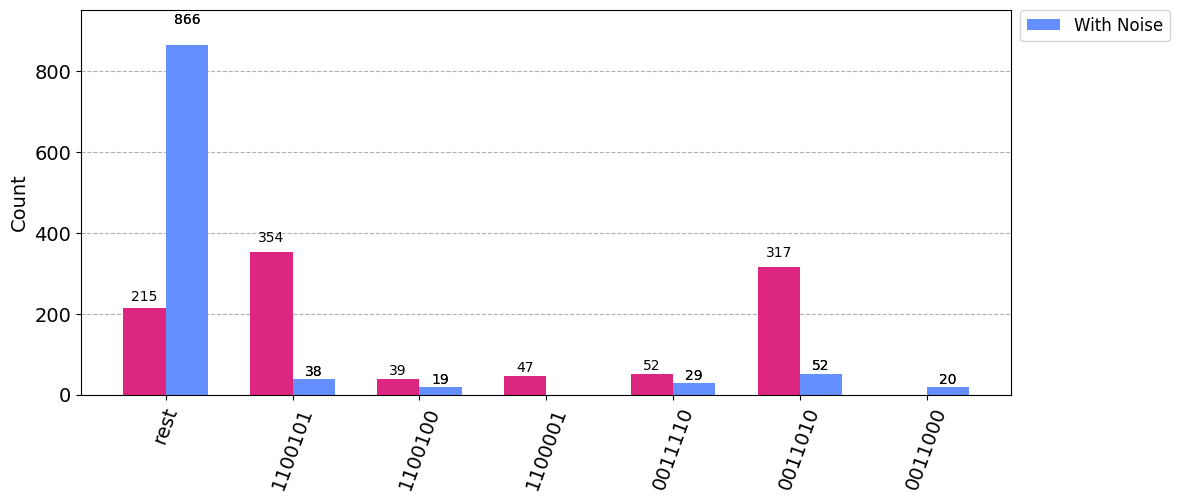
\includegraphics[width=0.5\textwidth]{result/[shots=1024]P=3}
%     }
%     \subfloat[$P=4$]{
%         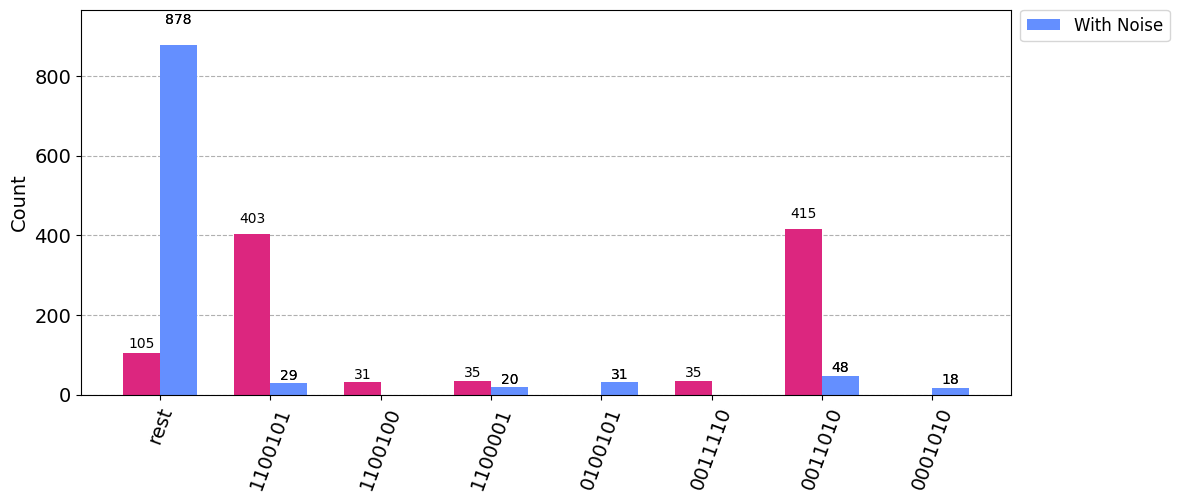
\includegraphics[width=0.5\textwidth]{result/[shots=1024]P=4}
%     }
    
%     \subfloat[$P=5$]{
%         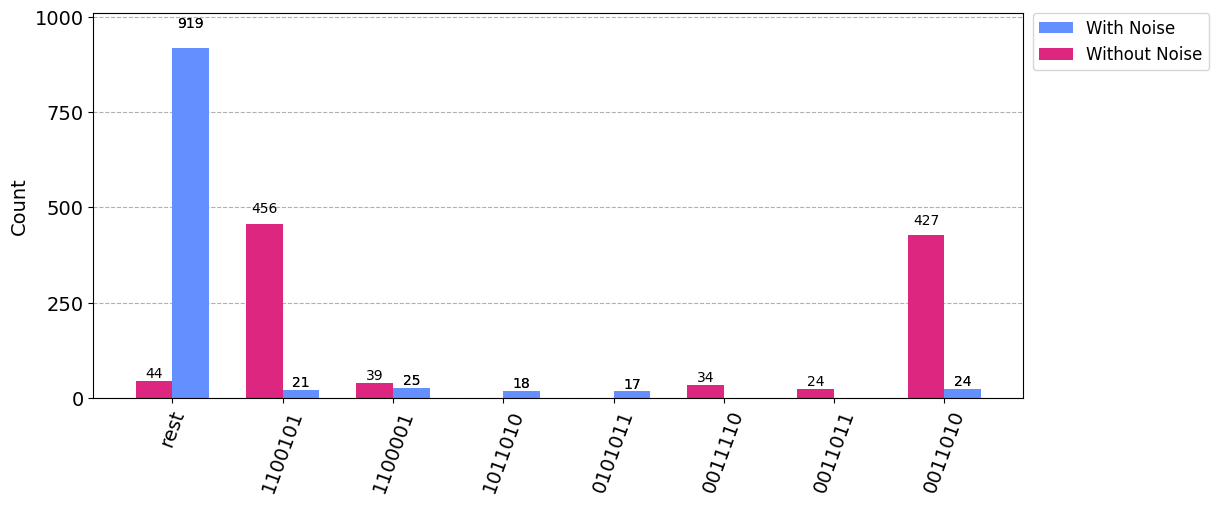
\includegraphics[width=0.5\textwidth]{result/[shots=1024]P=5}
%     }
%     \subfloat[$P=6$]{
%         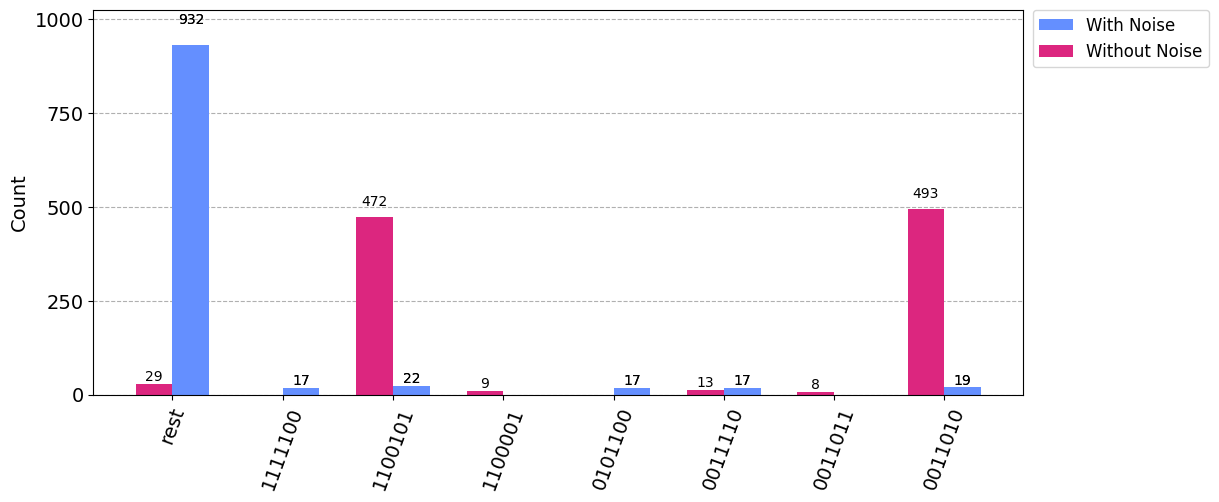
\includegraphics[width=0.5\textwidth]{result/[shots=1024]P=6}
%     }
%     \caption{1024 shots}
%     \label{fig:1024-shots}
% \end{figure*}

% \begin{figure*}[!htbp]
%    \centering
%     \subfloat[$P=1$]{
%         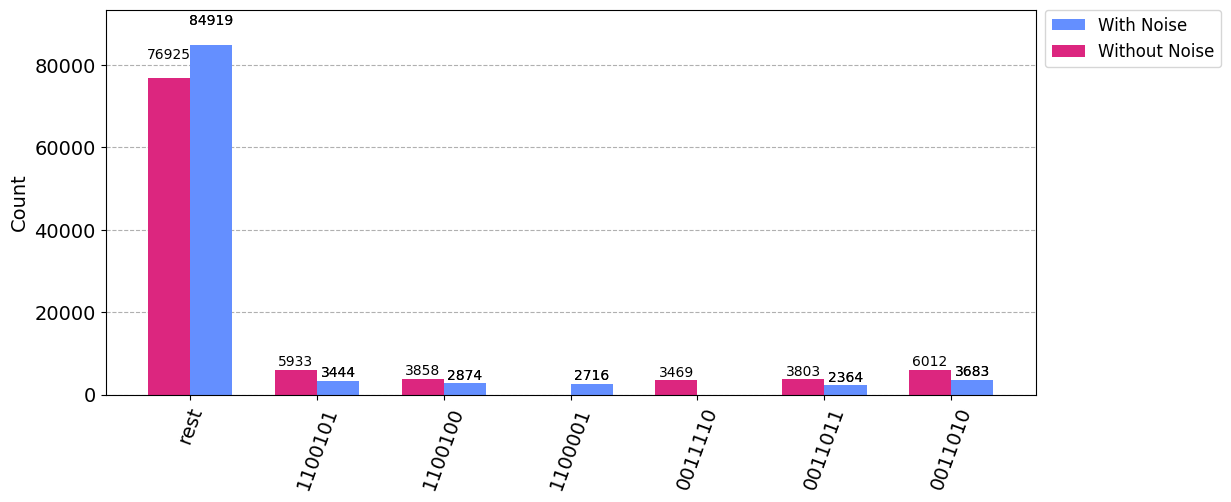
\includegraphics[width=0.5\textwidth]{result/P=1}
%     }
%     \subfloat[$P=2$]{
%         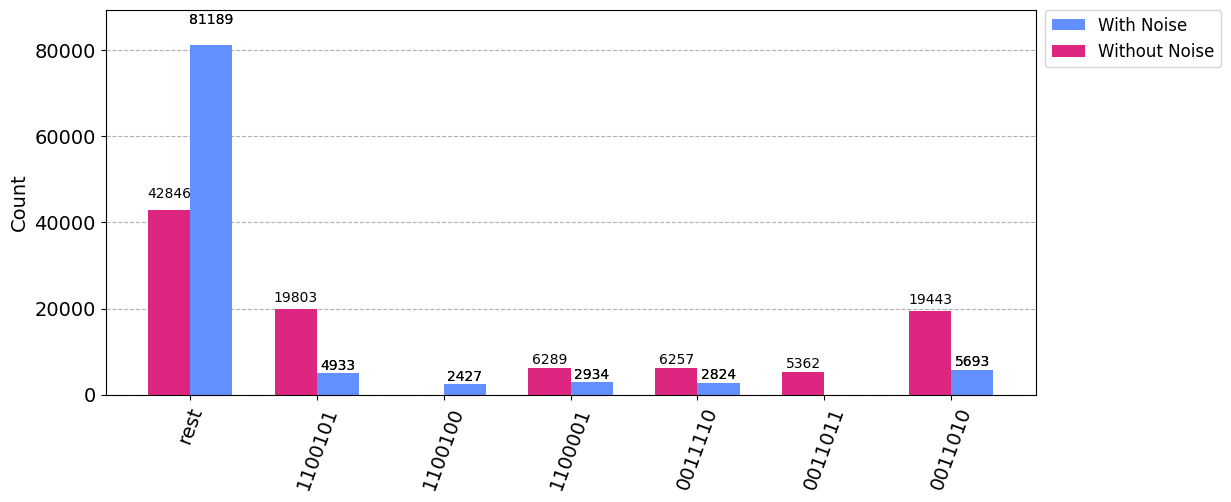
\includegraphics[width=0.5\textwidth]{result/P=2}
%     }
    
%     \subfloat[$P=3$]{
%         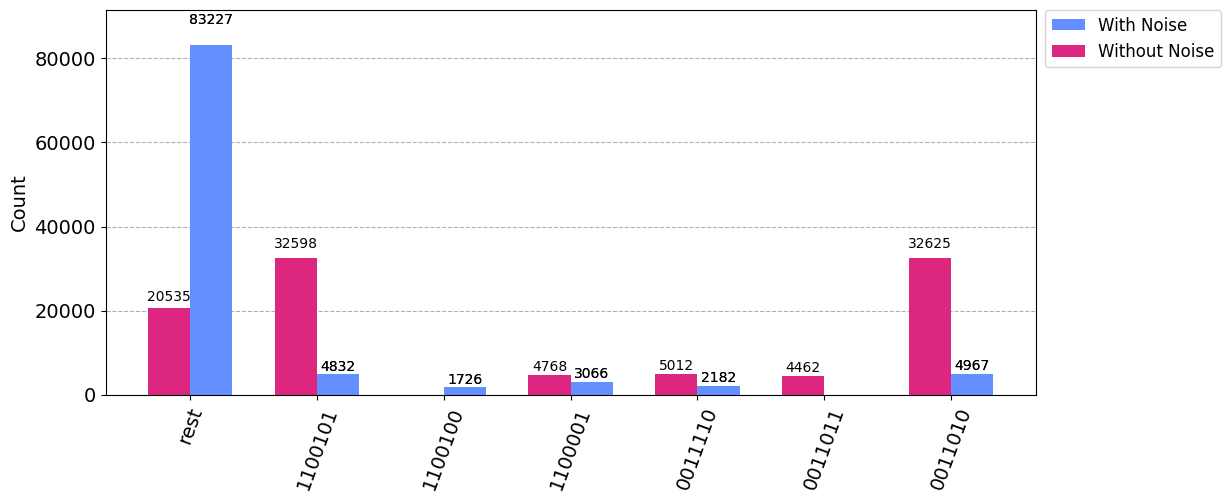
\includegraphics[width=0.5\textwidth]{result/P=3}
%     }
%     \subfloat[$P=4$]{
%         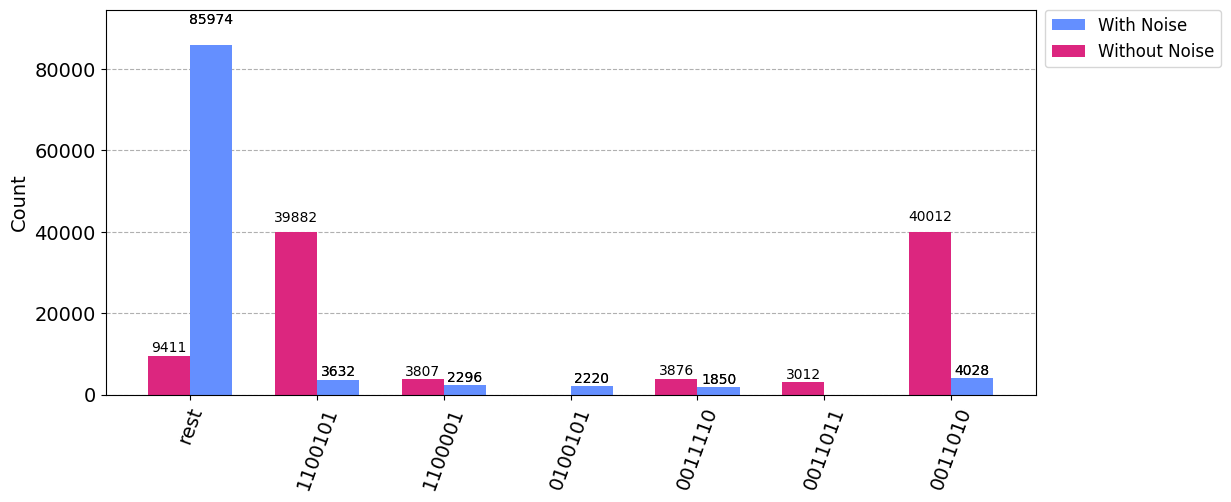
\includegraphics[width=0.5\textwidth]{result/P=4}
%     }
    
%     \subfloat[$P=5$]{
%         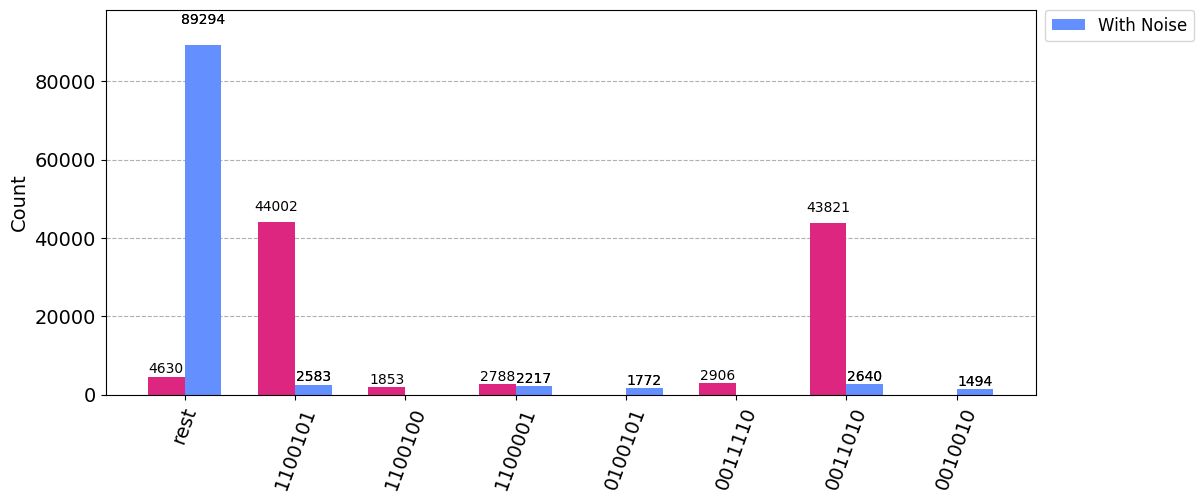
\includegraphics[width=0.5\textwidth]{result/P=5}
%     }
%     \subfloat[$P=6$]{
%         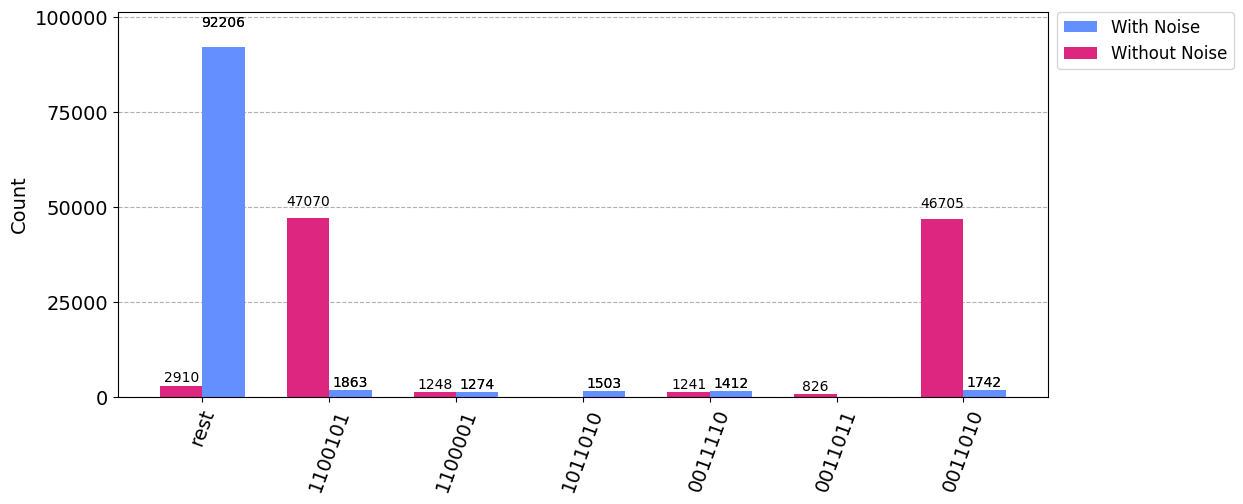
\includegraphics[width=0.5\textwidth]{result/P=6}
%     }
%     \caption{100000 shots}
%     \label{fig:100000-shots}
% \end{figure*}

%\clearpage